Darwin's theory of evolution through natural selection has been a cornerstone of
biology for over a century and a half. Yet, a quantitative theory of complexity
that could arise through Darwinian mechanisms has remained virtually unexplored.
To address this question, Valiant introduced a computational model of
evolution~\cite{Valiant:2009-evolvability}.  In his model, an organism is an
entity that computes a function of its environment.  There is a (possibly
hypothetical) \emph{ideal function} indicating the best behavior in every
possible environment. The performance of the organism is measured by how close
the function it computes is to the ideal. An organism produces a set of
offspring, that may have mutations that  alter the function computed. The
performance (fitness) measure acting on a population of mutants forms the basis
of natural selection. The resources allowed are the most generous while
remaining feasible; the mutation mechanism may be any efficient randomized
Turing machine, and the function represented by the organism may be arbitrary as
long as it is computable by an efficient Turing machine.

Formulated this way, the question of evolvability can be asked in the language
of computational learning theory. For what classes of ideal functions, $C$, can
one expect to find an evolutionary mechanism that gets arbitrarily close to the
ideal, within feasible computational resources? Darwinian selection is
restrictive in the sense that the only feedback received is {\em aggregate} over life
experiences. Valiant observed that any feasible evolutionary mechanism could be
simulated in the statistical query framework of Kearns~\cite{Kearns:1998}. In a
remarkable result, Feldman showed that in fact, evolvable concept classes are
exactly captured by a restriction of Kearns' model, where the learning
algorithm is only allowed to make \emph{performance queries}, \ie it produces a
hypothesis and then makes a query to an oracle that returns the (approximate)
performance of that hypothesis under the
distribution~\cite{Feldman:2008-evolvability}.\footnote{Feldman calls these
correlational statistical queries, because when working with boolean
functions with range $\{-1, 1\}$, the performance of any hypothesis is its
correlation with the ideal function.} P.  Valiant studied the evolvability of
real-valued functions and showed that whenever the corresponding weak
optimization problem, \ie approximately minimizing the expected loss, can be
solved by using a weak evaluation oracle, such an algorithm can be converted
into an evolutionary mechanism~\cite{Valiant:2012-real}. This implies that a
large class of functions -- fixed-degree real polynomials -- can be evolved
with respect to any convex loss function.

Direct evolutionary mechanisms, not invoking the general reductions of Feldman
and P. Valiant, have been proposed for certain classes in restricted settings.
Valiant showed that the class of disjunctions is evolvable using a simple set of
mutations under the uniform distribution~\cite{Valiant:2009-evolvability}.
Kanade, Valiant and Vaughan proposed a simple mechanism for evolving homogeneous
linear separators under radially symmetric distributions~\cite{KVV:2010-drift}.
Feldman considered a model where the ideal function is boolean but the
representation can be real-valued, allowing for more detailed feedback. He
presents an algorithm for evolving large margin linear separators for a large
class of convex loss functions~\cite{Feldman:2011-LTF}. P. Valiant also showed
that with very simple mutations, the class of fixed-degree polynomials can be
evolved with respect to the squared loss~\cite{Valiant:2012-real}.

Current understanding of biology (or lack thereof) makes it
difficult to formalize a notion of \emph{naturalness} for mutations in these
frameworks; in particular, it is not well understood how mutations to DNA
relate to functional changes in an organism. That said, the more direct
algorithms are appealing due to the simplicity of their mutations.  Also, the
``chemical computers'' of organisms may be slow, and hence, representations that
have low complexity are attractive.  In general, Feldman's
generic reduction from statistical query algorithms may use arbitrarily complex
representations (polynomial-sized circuits), depending on the specific algorithm
used.  In the remainder of the introduction, we first describe a particular
class of biological circuits, \emph{transcription networks}, that motivate our
study.  We then frame the evolutionary question in the language of computational
learning theory, summarize our contributions and discuss related work.

\subsection{Representation in Biology}

Biological systems appear to function successfully with greatly restricted
representation classes. The nature of circuits found in biological systems may
vary, but some aspects -- such as \emph{sparsity} -- are common.  Specifically,
the interacting components in many biological circuits are sparsely connected.
Biological circuits are often represented as networks or graphs, where the
vertices correspond to entities such as neurons or molecules and the edges to
connections or interactions between pairs of entities. For example, both neural
networks~\cite{Watts:1998} and networks of metabolic reactions in the
cell~\cite{Wagner:2001,Barabasi:2000} have been described by ``small-world''
models, where a few ``hub'' nodes have many edges but most nodes have few edges
(and consequently, the corresponding graphs have small diameter).  An associated
property observed in biological networks is \emph{modularity}: a larger network
of interacting entities is composed of smaller modules of (functionally related)
entities~\cite{Hartwell:1999}.  Both the ``small-world'' description and
modularity of biological networks are consistent with the more general theme of
sparsity.

\begin{figure}[!t]
\centering
\subfigure[~]{
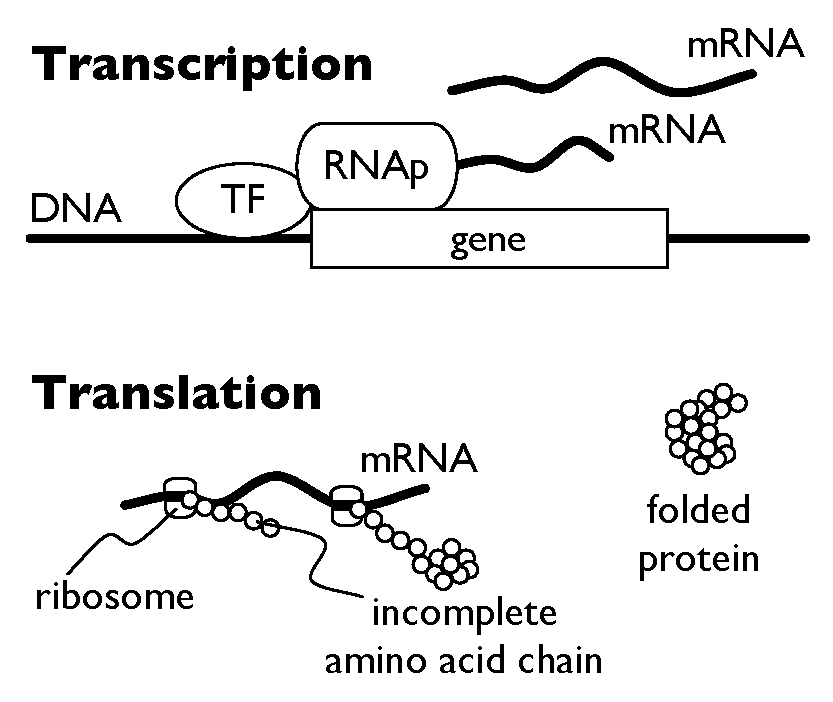
\includegraphics[width=0.35\textwidth]{figs/biology}
\label{fig:biology}
}
\subfigure[~]{
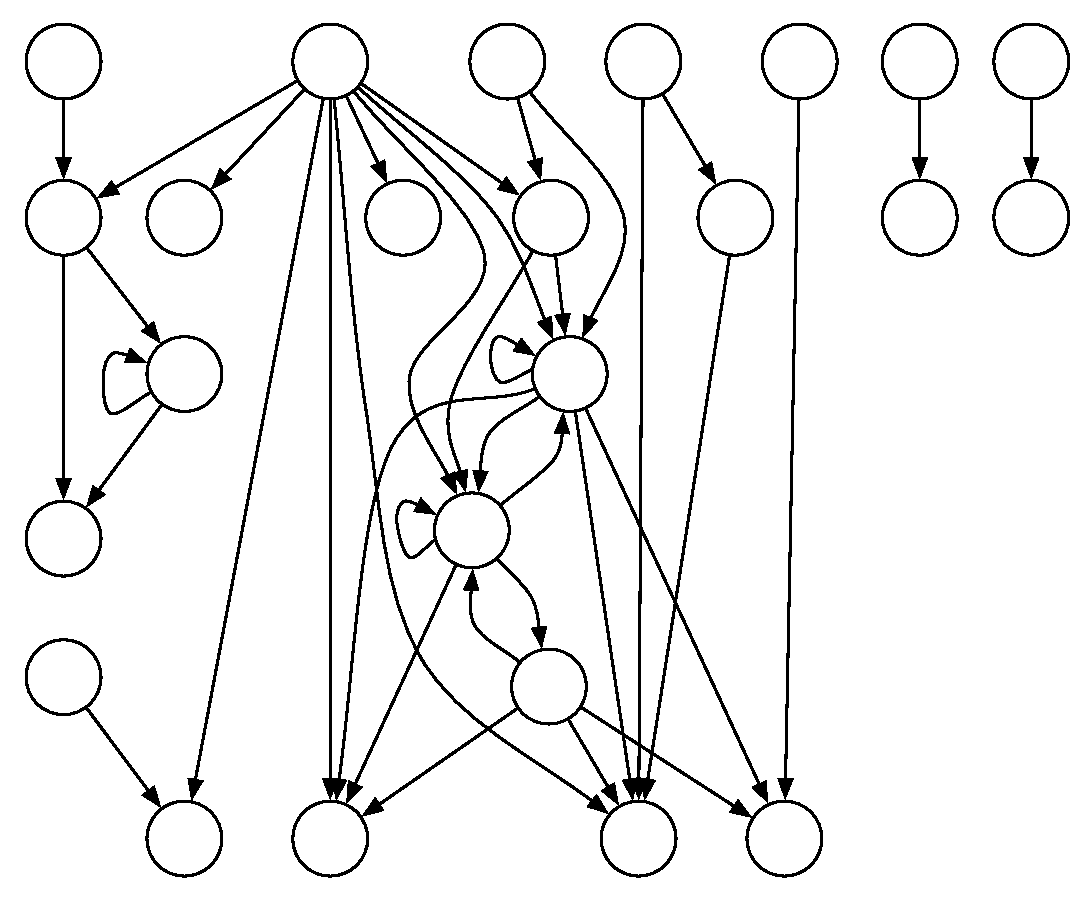
\includegraphics[width=0.35\textwidth]{figs/network}
\label{fig:network}
}
\caption{(a)~Schematic of transcription (top) and translation (bottom).
Here, a transcription factor (TF) binds to DNA close to a gene in a way that
increases gene expression by encouraging RNA polymerase (RNAp) to transcribe
the gene and so produce mRNA.  The mRNA is then translated by ribosomes to
produce sequences of amino acids that ultimately fold into proteins.
Only a small number of transcription factors
directly regulate any gene. Note that a transcription factor's action can also
decrease gene expression. For a more complete picture, see \eg~\cite{Alon:2006}.
(b)~Topology of the transcription network of respiration and redox reactions in
yeast. $X \rightarrow Y$ represents that transcription factor $X$ regulates the
expression of $Y$. Note that this real network has cycles.
Adapted from~\cite{Murray:2011}.}
\end{figure}

We focus on transcription networks, which are a specific class of networks of
interacting genes and proteins that are involved in the production of new
protein. Alon provides an accessible and mathematical introduction to
transcription networks and other biological circuits~\cite{Alon:2006}; below and
in Figure~\ref{fig:biology}, we present a simplified account that motivates this
work. Genes are \emph{transcribed} to produce mRNA, which is then
\emph{translated} into sequences of amino acids that ultimately fold into
proteins.\footnote{In reality, this is a dynamical system where the rates of
production are important. Note that this process need not be linear: a gene (mRNA
transcript) can be transcribed (translated) multiple times, not only in series
but also in parallel fashion.  We also ignore
other \emph{epigenetic} effects, \ie molecular modifications to DNA that do not
change its sequence but alter gene expression,~\eg the addition of methyl groups
to nucleotides in a way that physically blocks transcription.}
In a transcription network, a gene's transcription may be regulated by a set of
proteins called \emph{transcription factors}.
These transcription factors may increase or decrease a gene's transcription by
physically binding to regions of DNA that are typically close to the gene.
In natural systems, only a small number of transcription factors
regulate any single gene, and so transcription networks are sparsely connected.
For example, Balaji~\etal studied a yeast
transcription network of 157 transcription factors regulating 4,410 genes. They
observed this network to have 12,873 interactions (edges) where each gene was
regulated on average by about 2.9 transcription factors, the distribution of
in-degrees was well-described by an exponential fit, and only about 45 genes had
an in-degree of 15 or greater~\cite{Balaji:2006}.

The number of transcription factors varies from hundreds in a bacterium to
thousands in a human cell. Some transcription factors are always present in the
cell and can be thought of as representing a \emph{snapshot} of the
environment~\cite{Alon:2006}.
For example, the presence of sugar molecules in the environment may cause
specific transcription factors to be \emph{activated}, enabling them to regulate
the production of other proteins.  One of these proteins could be an
\emph{end-product}, such as an enzyme that catalyzes a metabolic reaction
involving the sugar. Alternatively, the transcription factor could regulate
another transcription factor that itself
regulates other genes -- we view this as intermediate computation -- and may
participate in further ``computation'' to produce the desired end-result.

While transcription networks may include cycles (loops), here for simplicity we
focus on systems that are directed acyclic graphs, and the resulting computation
can be viewed as a circuit. We illustrate a small, real transcription network in
Figure~\ref{fig:network}. These circuits are by necessity shallow due to
a temporal constraint, that the time required for sufficient quantities of
protein to be produced is of the same order of magnitude as cell-division
time.\footnote{Other kinds of networks, such as signaling networks, operate by
changing the shapes of proteins. The fact that these transformations are rapid
may allow for much larger depth. Note that fast conformational changes govern
how transcription factors directly process information from the environment in
order to regulate gene expression.  In our example, a sugar molecule binds to a
transcription factor and changes its shape in a way that alters its ability to
bind to DNA.} For example, Luscombe~\etal measured the shortest path length (in
number of intermediate nodes) between transcription factors and regulated genes
corresponding to terminal nodes (leaves) in a yeast transcription network. In
the static network, the mean such path length was 4.7 and the longest path
involved 12 intermediate transcription factors~\cite{Luscombe:2004}.

\subsection{Our Contributions}

First, our contribution is conceptual. We believe that the study of evolvability
from a computational standpoint will benefit by understanding the representation
complexity required to evolve a certain concept class. Motivated by the previous
discussion, in the case of transcription networks, it appears essential that the
representation used be a constant depth and fan-in (boolean or arithmetic)
circuit. Of course, any function that can be represented by such a circuit can
depend only on a constant number of input variables. We ask the
question, when we restrict attention to functions in a given class that depend
only on a constant number of variables, when can evolution succeed?

Second, we show that the class of sparse linear functions, those that depend
only on a constant number of variables, under a large class of smooth
distributions, can be evolved using sparse linear functions as representations,
when the performance is measured using squared error. The number of variables
used by the representations is larger than the number of variables in the
\emph{ideal function} and depends on the \emph{smoothness} parameter of the
distribution. According to our notion of $\Delta$-smooth $G$-nice distributions
(Defn.~\ref{defn:afghanistan}), the density function of a smooth distribution
is obtained by convolution of an arbitrary density with a product measure on
$[-\sqrt{3}\Delta, \sqrt{3}\Delta]^n$ (alternatively, drawing a point from the
smooth distribution is equivalent to drawing a point from an arbitrary
distribution and adding a (noise) vector from a product distribution). 

A linear function is represented by a weighted arithmetic circuit with only one
addition gate (alternatively, by a depth-two circuit with a layer of
multiplication gates and some constant inputs).\footnote{There is a natural
tradeoff between fan-in and depth, that may be useful, depending on which is the
more severe constraint.} Also, the number of generations required for evolution
to succeed depends polynomially on the sparsity $k$ of the target linear
function, the smoothness parameter $\Delta$ of the distribution and the inverse
of the target accuracy $\epsilon$, and has no dependence on the dimension $n$ of
the input space. The number of mutations explored at each generation depends
polynomially in $n$ and $1/\epsilon$. Thus, our result shows
\emph{attribute-efficient} evolvability of sparse linear functions, in the sense
of Littlestone~\cite{Littlestone:1988}. For the precise statement, see
Theorem~\ref{thm:sparse_linear} in Section~\ref{sec:sparse_linear}.

Valiant also proposed a stronger selection mechanism -- when natural selection
aggressively selects the (almost) best mutation, rather than merely a beneficial
one -- called evolution by optimization. Our second result requires a much
stronger distributional assumption -- the correlation $\corr(x_i, x_j) \leq
1/(2k)$ -- where $k$ is the sparsity of the target  linear function (see
Defn.~\ref{defn:bhutan}). Under such distributions, we show that under evolution
by optimization, sparse linear functions can be evolved by representations with
the same sparsity. The mechanism we propose and its analysis is inspired by the
greedy orthogonal matching pursuit algorithms in signal
processing~\cite{Donoho:2006-recovery,Tropp:2004-greed}. Unlike the previous
evolutionary algorithm, this one requires initialization, \ie the evolutionary
process begins with the $0$ function. As in the previous case, the number of
generations required depends polynomially on the sparsity $k$ of the target
linear function, the inverse of the accuracy parameter $\epsilon$, but has no
dependence on the total number of attributes $n$. The precise statement appears
as Theorem~\ref{thm:greedy} in Section~\ref{sec:greedy}.

\subsubsection*{Related Work}

The question of proper vs. improper learning has been studied in computational
learning theory. A separation between the two kinds is known, unless $\NP =
\RP$. However, most interesting PAC-learnable classes can be learned using
thresholds of low-degree polynomials, and do not seem to require the full
generality of polynomial-sized circuits.\footnote{For example, the classes of
$k$-CNF, $k$-term DNF, decision lists and low-rank decision trees, can all be
represented as PTFs.} In this context, Valiant's disjunction algorithm under the
uniform distribution~\cite{Valiant:2009-evolvability}, Kanade {\it et al.}'s
algorithm for homogeneous half-spaces under radially symmetric
distributions~\cite{KVV:2010-drift}, and P. Valiant's algorithm for linear
(polynomial) functions using squared loss~\cite{Valiant:2012-real}, are
\emph{proper} evolutionary mechanisms, \ie the representation used is from the
same class as the ideal function.  In the first two cases, it is straightforward
to show that if the target depends only on a constant number of variables, the
evolutionary mechanism also succeeds using representations that depend only on a
constant number of variables. Thus, attribute-efficient evolution can be
achieved.

The problem of learning sparse linear functions has been studied under various
names in several fields for many applications, \eg recovering sparse solutions
to (underdetermined) linear systems of equations~\cite{Donoho:2009-sparse}, or
recovering sparse representations with a redundant
dictionary~\cite{Mallat:2008,Elad:2010}; compressive sampling or compressed
sensing for sparse signal reconstruction~\cite{Candes:2008}; optimization with
regularization or sparsity-inducing penalties in machine
learning~\cite{Bach:2012}; sparse coding for learning an overcomplete
basis~\cite{Olshausen:1997}, or for denoising in image and video
processing~\cite{Elad:2010}. This area is too vast to review here; Bruckstein
\emph{et al.} have an excellent survey~\cite{Donoho:2009-sparse}.  Learning the
sparsest linear function is equivalent to finding the sparsest solution to a
system of linear equations (assuming there is no noise in the data). In general,
this problem is $\NP$-hard and the currently best-known approximation factor
depends on the norm of the pseudo-inverse of the matrix~\cite{Natarajan:1995}.
Thus, some assumption on the distribution seems necessary. Our evolution based
on optimization algorithm (Section~\ref{sec:greedy}) is essentially the greedy
orthogonal matching pursuit algorithm of Tropp~\cite{Tropp:2004-greed} and
Donoho \emph{et al.}~\cite{Donoho:2006-recovery}, cast in the language of
evolvability; these algorithms are also known in statistical modeling as forward
stepwise regression~\cite{Daniel:1999,Hastie:2001}.

Finally, the question of \emph{attribute-efficient} regression in the PAC (or
SQ) model is a natural one. Here, the goal would be to design a polynomial time
algorithm for producing an $\epsilon$-accurate linear function, with sample
complexity that is polynomial in the sparsity $k$ of the target function and the
inverse of the target accuracy $\epsilon$, and only polylogarithmic in $n$, the
total number of attributes. Under mild boundedness assumptions on the
distribution, this can be achieved by setting up an $L_1$-regularized
optimization problem; the output classifier may not be sparse in light of the
$\NP$-hardness result mentioned above. We note that under the distributional
assumption made in this paper, finding the \emph{sparsest} linear function that
fits the data is also easy in the PAC/SQ setting, since the solution to the
optimization problem in this case is unique. The focus in our work is different,
namely showing that simple evolutionary mechanisms can succeed, while using
representations that are themselves sparse linear functions at all times.

\subsubsection*{Organization}

In Section~\ref{sec:notation}, we give an overview of Valiant's evolution model
and describe the concept classes and class of distributions considered in this
paper.  Section~\ref{sec:algorithms} contains the mechanisms for evolving sparse
linear functions. We conclude in Section~\ref{sec:conclusion} with some
discussion and directions for future work.
